%----------------------------------------------------------------------------------------
%   BEER PONG RULES: MAIN
%----------------------------------------------------------------------------------------
%\documentclass[rules] % Custom document class
\documentclass[11pt, oneside,letterpaper]{article}

%----------------------------------------------------------------------------------------
%	PACKAGES AND OTHER DOCUMENT CONFIGURATIONS
%----------------------------------------------------------------------------------------

% Packages
    \usepackage[english]{babel}
    \usepackage{lmodern}
    \usepackage{graphicx}
    \usepackage{titlesec}
    \usepackage[left=3.04cm, right=2.54cm, bottom=2.54cm]{geometry}
    \usepackage{changepage} % indenting subsubsections
    \usepackage{framed}
    \usepackage{fancyhdr}
    \usepackage{enumitem}
    \usepackage{yfonts}
    \usepackage{titletoc}
    \usepackage{float} % float option [H] for better floats for figures
    \usepackage{siunitx} % Consistent unit typesetting

% Add US imperial units macro based on SI units
    \let\DeclareUSUnit\DeclareSIUnit
    \let\US\SI
    % Declare Units
        \DeclareUSUnit\ounce{oz}
        \DeclareUSUnit\inch{in}
        \DeclareUSUnit\feet{ft}
        \DeclareUSUnit\USoz{\text{US fl oz}}

% Set a Title font to gothic
    \font\titleFont = ygoth at 50pt

% Defines a new command for the horizontal lines, change thickness here
    \newcommand{\HRule}{\rule{\linewidth}{0.5mm}} 

% Page Header and Footer
    \pagestyle{fancy}
    \setlength{\headheight}{14pt}

    \fancyhf{}
    \rhead{\leftmark}
    \lhead{House Beer Pong Rules}
    \rfoot{Page \thepage}
    \renewcommand{\headrulewidth}{0.5pt}

% Sectioning customization
    \renewcommand{\thesection}{\Roman{section}} 
    \renewcommand{\thesubsection}{\Roman{section}.\Roman{subsection}}

    \titleformat{\section}{\titlerule[2pt]\vspace{.8ex}\Large\bfseries}{\thesection.}{.5em}{\vspace{0pt}}
    \titleformat{\subsection}{\large\bfseries}{\Roman{subsection}.}{.5em}{\vspace{0pt}}

    \titlespacing*{\section}{-1cm}{0.2cm}{0cm}
    \titlespacing*{\subsection}{-0.5cm}{1em}{0.5em}

% Graphics Path
    \graphicspath{{Figures/}}

% referencing sections
    \setcounter{secnumdepth}{3}

% footnote numbering
    \renewcommand{\thefootnote}{\fnsymbol{footnote}}

% ToC depth
    \setcounter{tocdepth}{2} %	2 = Up to subsection layer

    \titlecontents{section}
    [0em] % i
    {\smallskip}
    {\bfseries \thecontentslabel\enspace}%\thecontentslabel
    {\hspace*{-5.5em}}
    {\titlerule*[1pc]{.}\contentspage}%]

    \titlecontents{subsection}
    [2.5em] %
    {\smallskip}
    {\thecontentslabel\enspace}%\thecontentslabel
    {\hspace*{7.12em}}
    {\titlerule*[1pc]{.}\contentspage}

\usepackage{hyperref}
 % Remove to just use custom class

\begin{document}

%----------------------------------------------------------------------------------------
% Titles
%----------------------------------------------------------------------------------------
		\begin{titlepage}

		\center % Center everything on the page

	%----------------------------------------------------------------------------------------
	%	HEADING SECTIONS
	%----------------------------------------------------------------------------------------
		\textsc{\large	On Writ of  the Disputatorium to the }		\\ [0.3cm]
		\textsc{\Large INSTITUTION OF DRINKING }					\\ [0.3cm]
		\textsc{\large on Beer Pong Rules and Regulations}		 \\ [0.3cm]

	%----------------------------------------------------------------------------------------
	%	TITLE SECTION
	%----------------------------------------------------------------------------------------
		
		\HRule \\[0.4cm]
		{\titleFont The Rule Book} \\ % Title of your document
		\HRule \\
		\Large\textsc{A codex of utmost authority}\\
		\large \textit{2nd Edition}\\[0.5cm]
		
		
		
	%----------------------------------------------------------------------------------------
	%	AUTHOR SECTION
	%----------------------------------------------------------------------------------------
			
		%\normalsize \emph{Authors:}
        % Author's \textsc{Name}	
		
	%----------------------------------------------------------------------------------------
	%	LOGO SECTION
	%----------------------------------------------------------------------------------------
		\vspace*{\fill}
		\begin{figure}[h]
			\centering
			\includegraphics[width=0.3\textwidth]{crestNA.png}
		\end{figure}
		\textit{Confidunt in cervisia nobis}% In beer we trust 
		
	%----------------------------------------------------------------------------------------
	\vspace*{\fill}
	 Promulgated this first month of the year \textbf{MMXXI} \\ under the grace of his lord and saviour, ethanol.

	\end{titlepage}


% blank and ToC
	\newpage\thispagestyle{empty}
	\emph{This page is intentionally no longer blank}

% Signatures
\newpage\thispagestyle{empty}
\textbf{This Document has been read in it's entirety(ish) and approved by: }

\vspace{1.5cm}
\noindent Name: \hrulefill \\[1cm]
Date: \rule{1.5in}{0.5pt}
\noindent Signature: \hrulefill \\[1.5cm]

\noindent Name: \hrulefill \\[1cm]
Date: \rule{1.5in}{0.5pt}
\noindent Signature: \hrulefill \\[1.5cm]

\noindent Name: \hrulefill \\[1cm]
Date: \rule{1.5in}{0.5pt}
\noindent Signature: \hrulefill \\[1.5cm]

\noindent Name: \hrulefill \\[1cm]
Date: \rule{1.5in}{0.5pt}
\noindent Signature: \hrulefill 


% Table of Contents
	\newpage\thispagestyle{empty}
	\tableofcontents \thispagestyle{empty}
	\newpage

%----------------------------------------------------------------------------------------
%	Introduction
%----------------------------------------------------------------------------------------
	\setcounter{page}{1} % Set counter to page 1
	\begin{center}
		\textbf{Preface} \\
	\end{center}
		Beer pong, Sometimes called Beirut is a game played with ping pong balls, Solo cups and beer.
        The aim is to throw the ping pong balls into your opponent(s) solo cups that traditionally contains beer.
        When a ball lands in a cup, the cup is removed and the thrower's opponent(s) drinks.
        The first person or team to successfully make their opponent(s) drink all their cups wins.

		There are many styles of playing.
        Here we present the House rules of 3727 for the ultimate beer pong game experience. 
        This text is organized into four sections: the setup, the gamplay, special shot types and then extra miscellaneous Rules.

%----------------------------------------------------------------------------------------
% Input body files
%----------------------------------------------------------------------------------------

%--------------------------------------------------------
% BEER PONG RULES: SETUP SECTION
%--------------------------------------------------------
\section{Setup}\label{sec:SETUP}
	\subsection{Cup Formation}\label{ssec:CupFormation}
		\begin{enumerate}[label=(\roman*), ref=\roman*]
            \item \label{itm:CF,solocups} Each player's rack is to be made up of 10 red \US{18}{\USoz} solo cups.
                See \hyperref[fig:solocup]{Figure \ref*{fig:solocup}} for the regulation cup specifications. 
            \item \label{itm:CF,triangle} The starting rack is a tight equilateral triangle with the base towards the player's table edge and the tip towards the opponent. 
            \item \label{itm:CF,position} The rack's back edge is to be at least two finger widths from the edge but no more than 4 and centred from side to side. 
            \item \label{itm:CF,kissing} Solo Cup rims must be ``kissing". There should be minimal spaces in between the cups but not so close as to lean, tilt, or overlap onto their neighbouring cups. 
        \end{enumerate}
        \begin{figure}[H]% Shows a single rack setup
            \centering
            \def\svgwidth{0.4\columnwidth}
            \input{Figures/startrack.pdf_tex}
            \caption{Diagram of a full 10 rack of cups, centred on the table. The arrow points towards the opponent's rack. The hashed middle cup is the bitch cup (see \hyperref[ssec:BitchCup]{Section \ref*{ssec:BitchCup}}).}
            \label{fig:therack}
        \end{figure}
	\subsection{Cup Content}\label{ssec:CupContent}
        \begin{enumerate}[label=(\roman*), ref=\roman*]
            \item \label{itm:CC,filling} Cups are to be filled to a minimum that stops the moving and sliding when a ball is sunk into the cup. 
            \item \label{itm:CC,w_vs_l} The physical content of the cup is either water or liquor.
                \begin{enumerate}[label=(\alph*), leftmargin=2cm]
                    \item Water Cups: Water is put into the cups following \hyperref[itm:CC,filling]{Section \ref*{ssec:CupContent}.\ref*{itm:CC,filling}} regulations.
                    \item Drink Cups: Drinks are put into the solo cups following \hyperref[itm:CC,filling]{Section \ref*{ssec:CupContent}.\ref*{itm:CC,filling}} regulations and budget costs...
                \end{enumerate} 
            \item \label{itm:CC,rinse} A cup of water will be provided to the players to rinse the balls off when playing with beer. This is for sanitary reasons. 
        \end{enumerate}        
    \subsection{The Balls}\label{ssec:Balls}
        \begin{enumerate}[label=(\roman*), ref=\roman*]
            \item \label{itm:Balls,num} The game is played with 2 \US{1.57}{\inch} or \US{40}{\milli\metre} diameter, Ping Pong Balls (see \hyperref[fig:solocup]{Figure \ref*{fig:solocup}}).
            \item \label{itm:Balls,dents} The balls must have no dents. 
            \item \label{itm:Balls,bounce} The balls must be checked to have the same elasticity (bounce). 
            \item \label{itm:Balls,texture} The texture of the balls must be consistent between the two; to the player's standards. This is for consistency of throwing. 
        \end{enumerate}    
	\subsection{The Cup}\label{ssec:Cup}
        \begin{enumerate}[label=(\roman*), ref=\roman*]
            \item \label{itm:Cup,dim} The solo cups are to be red, \US{18}{\USoz} and have the dimensions as seen in \hyperref[fig:solocup]{Figure \ref*{fig:solocup}}. 
            \item \label{itm:Cup,broken} Cups should not be used if broken or cracked in any way. Change this cup out. 
            \item \label{ssec:Cup,rinsing} Cups should be rinsed before a game in both water and drink versions before play. Cups can get quite gross. 
        \end{enumerate}
        \begin{figure}[H]
            \centering
            \def\svgwidth{\columnwidth}
            \input{Figures/CupDimensions.pdf_tex}
            \caption{Dimensions of a regulation \US{18}{\ounce} Solo Cup and Regulation ping pong ball.}
            \label{fig:solocup}
        \end{figure}
	\subsection{Teams}\label{ssec:Teams}
		\begin{enumerate}[label=(\roman*), ref=\roman*]
            \item \label{itm:teams,options} There are two options to play beer pong: single or doubles. 
                \begin{enumerate}[label=(\alph*), leftmargin=2cm]% Singles vs doubles
                    \item \textbf{Singles:} Beer pong can played as singles where for each rack there is one player.
                        This player will throw two balls each go. 
                        The two balls (first and second throw) are independent of rules such as ``on-fire" and ``bounce".
                    \item \textbf{Doubles:}	This is a variation still played with two ping pong balls where each member of the team now throws a single ball.
                        Again, each ball is considered independent for rules such as ``on-fire" and ``bounce" but this time it is by player and not throw order.
                \end{enumerate} 
            \item \label{itm:teams,choosing} There are no set rules for how teams are formed. Figure it out bud. 
        \end{enumerate}
	\subsection{The Table}\label{ssec:Table}
        \begin{enumerate}[label=(\roman*), ref=\roman*]
            \item \label{itm:Table,sides} The table is split into two sides down the midline (see \hyperref[fig:table]{Figure \ref*{fig:table}}).
			    The opponents take opposite sides of the table. 
			    From the midpoint on the table in the direction the player is considered ``their side". 
            \item \label{itm:Table,switch} If multiple games in a row are being played by the same players, they must switch sides every game. 
            \item \label{itm:Table,length} The table must be at least \US{5}{\feet} long. 
        \end{enumerate}
        \begin{figure}[H]
            \centering
            \def\svgwidth{\columnwidth}
            \input{Figures/table.pdf_tex}
            \caption{The table viewed from the top showing two racks, accepted throwing zones, the midpoint, and the 2 fingers from the edge that the rack has to be.}
            \label{fig:table}
        \end{figure}
		
\section{Gameplay}\label{sec:Gameplay}

    \subsection{Deciding Throw Order (eye-to-eye) (snake-eyes)}\label{ssec:Order}
		\subsubsection{}\label{sssec:Order,ete1}
			Each opposition will start with a single ball each. Maintaining eye contact with the other thrower, the player will attempt to throw into the cups. 
            \begin{enumerate}[label=(\alph*), leftmargin=2cm]% Singles vs doubles
                \itemsep -1.25em 
                \item Singles: Each player gets a ball and throw continuously at the same time until one player sink the ball and the other misses.\\
                \item Doubles: 	The players switch off on each team each throw. The player who shit last on the team will throw eye-to-eye first.
            \end{enumerate}
		\subsubsection{}\label{sssec:Order,ete_remove}
			During eye-to-eye, no cups are removed when balls are sunk. This includes intermediate ties.
		\subsubsection{}\label{sssec:Order,ete_ties}
			If both balls are sunk on the same eye-to-eye throw, then nothing is decided.
            Even if one ball is sunk faster on the throw. Eye-to-eye continues until one player sinks the ball and the other does not.
		\subsubsection{}\label{sssec:order,ete_2ball}
			Once the game of eye-to-eye is won, the winner gets possession of both balls to begin his first real throw.
        \subsubsection{}\label{ssec:order,bitchcup}
            The bitch cup has no effect in deciding play order so a ball sunk in the bitch counts as sunk ball.
	
	\subsection{Throwing}\label{ssec:Throwing}
		\subsubsection{}\label{sssec:Throwing,stand_behind}
			When throwing player must be directly behind their pane of play of the table (see Figure \ref{fig:table}).
            Shots taken from standing to far in front of the edge are void. You do not get to throw again this turn.
		\subsubsection{}\label{sssec:Throwing,wrists}
			 Wrists will always stay behind the pane of play when throwing.
             If the wrist goes over the table edge then the shot is void. You do not get to throw again this turn.
		\subsubsection{}\label{sssec:Throwing,feet}
            Unless performing a suitable trick-shot, both feet must remain on the ground in the accepted throwing zone (see Figure \ref{fig:table}).
		\subsubsection{}\label{sssec:Throwing,bumping_table}
			When throwing, no player can touch/bump/move the table in anyway that effects the balls outcome.
		\subsubsection{}\label{sssec:Throwing,possesion}
			The player/team may not throw until both balls are thrown by the opponents.

	\subsection{Defending}\label{ssec:Defending}
		\subsubsection{}\label{sssec:Defending,blowing}
			When the ball hits the cup, sometimes it will spin on the rim/insides for a time.
            This balls may be "blown" by  blowing into the cup with your mouth.
            Everyone blows.
            Fingering is not allowed.
		\subsubsection{}\label{ssec:Defending,blowing_voids}
			If the ball has touched water it may not be blown out and the cup must be removed from play and drinking must occur for that cup.
		\subsubsection{}\label{sssec:Defending,blowing_times}
			The player is not limited to the number of times he/she can blow. More blowing makes for a fun night...
		\subsubsection{}\label{sssec:Defending,pysycedout}
			The defending team may do most anything they want to distract the other team except for blocking visual or physical path to the cups.
            Player must not cross the plane of play while doing this (see Figure \ref{fig:table}).
		\subsubsection{}\label{sssec:Defending,balltouching}
			Except in a bounce shot (see \ref{ssec:BounceShots}) opponents are not allowed to swipe or grab the ball until it has bounced or sank into a cup.
            \footnote{The opponents may grab after the first bounce no matter where the bounce occurred.}
		
	\subsection{Sinking A Ball}\label{ssec:Sinking}
		\subsubsection{}\label{sssec:Sinking,def}
			A ball is considered to be sunk when it has touched the liquid inside the cup.
            Once this has occurred, then the cup is marked for removal. 
		\subsubsection{}\label{sssec:Sinking,removal}
			Once a ball has been sunk, it is removed from the cup before the player throws their next ball.
            This is the responsibility of the defender given a reasonable time frame.
		\subsubsection{}\label{sssec:Sinking,non-removal}
			If the ball is not removed that the next ball goes into the same cup and bounces out \textit{Due to the other ball being in there}, the ball will count as sunk.
		\subsubsection{}\label{sssec:Sinking,cups_away}
			The cups are removed only after both balls are thrown in case of bomb and island shots.
		\subsubsection{}\label{sssec:Sinking,knockedover}
			A ball knocking over/knocking off and spilling it's contents counts as a sunk ball. 
		\subsubsection{}\label{sssec:Sinking,cups_drinking}
			At the end of the opponents turn, the players remove the sunk cups and take appropriate drinks.

	\subsection{Reracks}\label{ssec:Rerack}
		\subsubsection{}\label{sssec:Rerack,number}
			During the game, each team can request a rerack once.
		\subsubsection{}\label{sssec:Rerack,notallowed}
			Players cannot ask for a rerack when it is not their turn, after throwing their first ball, or on balls back (including on fire).
            I.e only at the start of their go.
		\subsubsection{}\label{sssec:Rerack,pop_forms}
			Popular formations are shown in figure \ref{fig:rerack_forms}.
            You are not limited to these formations but are provided here for convenience and to avoid misunderstandings. 
		\subsubsection{}\label{sssec:Rerack,centering}
			All rerack formations should be centred on the table from side to side and two fingers from the players edge but no maore than 4.
		\subsubsection{}\label{sssec:Rerack,Island}
			A player may not request a rerack that would give them an island cup.
		\subsubsection{}\label{sssec:Rerack,4cupdeep}
			A player may not request a rerack that puts the cups closer then the tip cup of a full rack.
            i.e. 4 cups deep towards the opponent.
		\subsubsection{}\label{sssec:Rerack,autoreracks}
			A player gets an automatic rerack at 2 and 1 cups.
            The two cups can be placed parallel or orthogonal to the pane of play.
            The last cup rerack is centred on the table.

    \begin{figure}
        \centering
        \includegraphics[width=0.75\textwidth]{rerack_formations.png}
        \caption{Popular rerack formations}
        \label{fig:rerack_forms}
    \end{figure}

	\subsection{Balls Back, On-fire, Roll Backs}\label{ssec:BallsBack}

    \noindent\textbf{Balls Back}
		\subsubsection{}\label{sssec:BallsBack,bothin}
			If a player or team gets both balls in on the same turn, then both balls will be given back to the thrower(s) to continue the round.
            This can happen multiple times.
		\subsubsection{}\label{sssec:BallsBack,onfire_combine}
            If a player gets balls back but also onfire(see section \ref{sssec:BallsBack,onfire} to section \ref{sssec:BallsBack,onfire_calling}), The player will play the balls back shot first and continues taking the balls back following the \ref{sssec:BallsBack,bothin} Section rules.
            The player then still gets the ball back to play the on fire shots (Section \ref{ssec:BallsBack}) after losing balls back.

    \noindent\textbf{On-fire}
		\subsubsection{}\label{sssec:BallsBack,onfire}
			If a player gets two shots sunk in a row with the same ball (1st throw and 2nd throw for singles)  the the player can call heating up.
            If a third is sunk with the same ball, the player is considered to be "on-fire" and will get the ball back. 
		\subsubsection{}\label{sssec:BallsBack,onfire_reset}
			All three shots do not have to occur in the same turn but must be in the same game. Remember the shots must be consecutive to be valid "on-fire" throws.
		\subsubsection{}\label{sssec:BallsBack,onfire_multiple}
			"On-fire" lasts as long as the balls are consecutively being sunk. 
		\subsubsection{}\label{sssec:BallsBack,onfire_calling}
			The player that is heating up must call heating up or they will not be on fire and get the balls back even if they get it in.
		
    \noindent\textbf{Steal Backs}
		\subsubsection{}\label{sssec:BallsBack,stealback}
			If the balls have not touched a horizontal surface other than the table, the throwers may "steal the ball" by grabbing it before the defenders.
            They get another throw with that ball.
		\subsubsection{}\label{sssec:BallsBack,stealback_multi}
			A steal back may occur multiple times in a row.
            The player must use the non-dominant hand trick shot multiple times. This is the only exception to repeating trick shots.
        \subsubsection{}\label{sssec:BallsBack,stealback_redo}
            The first shot is void and the steal back shot will contribute to onfire streaks and balls back double-ins.

	\subsection{The Bitch Cup}\label{ssec:BitchCup}
		\subsubsection{}\label{sssec:BitchCup,def}
			The bitch cup is defined ONLY for a full rack as the centre most cup.
            See Figure \ref{fig:therack} for clarity. If this cup is sunk first, it does not not count as sunk.
		\subsubsection{}\label{sssec:BitchCup,rem}
			If the throwers bitch cup is still in play then the throwers bitch cup is removed instead.
            If the bitch cup is already gone, the foremost cup (closest to opponent) of the thrower is taken left to right.
		\subsubsection{}\label{sssec:BitchCup,song}
			If a bitch cup is sunk, Move Bitch by Mystikal must be played.
        \subsubsection{}\label{sssec:BitchCup,redemption}
            Called \emph{Growing a pair} a player may call redemption if they or their partner still have a ball to throw.
            If the team gets their second shot in the bitch again, no cups are removed.
        \subsubsection{}\label{sssec:BitchCup,redemptionFail}
            f the team calls redemption and gets it into a non-bitch cup, that cup is removed from the throwers rack as well.

	\subsection{Winning The Game/Redemption}\label{ssec:Winning}
		\subsubsection{}\label{sssec:Winning,lastcup}
			If a team makes their last cup, the other team loses and has the chance to perform a "redemption shot"
		\subsubsection{}\label{sssec:Winning,redemption}
			The team throwing the redemption shot must make the number of shots in any cup as their opponents got into their final cup to be successful.
            This could be more than 2 as balls back is still valid on the final cup.
		\subsubsection{}\label{sssec:Winning,onfire}
			Each ball is considered to be "on fire" when starting to throw redemption shots and will follow the same rules until the thrower misses.
		\subsubsection{}\label{sssec:Winning,specialshot}
            You must not use a bonus cup to put the other team into redemption.
		\subsubsection{}\label{sssec:Winning,drinking}
			A player/team may not win unless they have all their removed cups drank to completion or if playing with water cups, drinks have been appropriately drank for. 
		\subsubsection{}\label{sssec:Winning,death/killcups}
			An automatic win for the throwers can occur if a ball is sunk in a cup that was forgotten to be removed from the rack previously.
            No redemption
		\subsubsection{}\label{sssec:Winning,knockovers}
			An automatic win will occur if the opposing team knocks their entire rack off the table by accident (or on purpose?).
		\subsubsection{}\label{sssec:Winning,shutout}
			A shutout occurs when a player/team sinks there a ball in their opponents final cup while no cups are removed from the other rack.
            There is no redemption chance for the defenders.
            The defenders must sit under the table for the next entire next match of beer pong.
		\subsubsection{}\label{sssec:ResidentWins}
			A resident of 3727 may invoke this rule and they automatically win the game.
            The other team must drink their rack or finish their drink.
        \subsubsection{}\label{sssec:Winning,no.Redemtions}
            There is no limit to the number of redemptions the players may use.
			

%--------------------------------------------------------
% BEER PONG RULES: SPECIAL SHOTS SECTION
%--------------------------------------------------------
\section{Special Shots}\label{sec:SpecialShots}
	\subsection{Celebrity Shot}\label{ssec:CelebShot}
		\begin{enumerate}[label=(\roman*), ref=\roman*]
            \item \label{sssec:CelebShot,number} A celebrity shot may only be called once a game.
            \item \label{sssec:CelebShot,finalcup} The Thrower may not use a celebrity shot to put their opponents into redemption.
            \item \label{sssec:CelebShot,redemption} A player may use a celebrity shot for a redemption shot.
            \item \label{sssec:Celeb,special} A celebrity may use a special shot. Though no extra bonuses (just the regular bonus cup rules) are given.
        \end{enumerate}
    \subsection{Double or Nothing (Optional Rule)}\label{ssec:Double-or-Nothing}
		\begin{enumerate}[label=(\roman*), ref=\roman*]
            \item \label{sssec:DN,calling} A player may call Double-or-Nothing once per game when at least one ball has been sunk successfully.
            \item \label{sssec:DN,combo} The thrower will not get any more bonus cups for combining double-or-nothing with any other special shot, including on-fire or steal-backs.
            \item \label{sssec:DN,condition} Once the player has thrown both balls, the player calling double-or-nothing will get one ball back to throw again.
                If this ball is sunk in an already sunk cup, the thrower gets bonus cups of their choice equal to the number of balls sunk.
            \item \label{ssec:DN,condition} If the double-or-nothing shot is a miss, the previous balls do not count as sunk anymore.
                No cups are removed from the rack.
            \item \label{sssec:DN,redemption} Like other special shots, you are not allowed to use this to put your opponent into redemption.
        \end{enumerate}
	\subsection{Trick Shots}\label{ssec:TrickShots}
        \begin{enumerate}[label=(\roman*), ref=\roman*]
            \item \label{sssec:trickShots,deff} A trick shot modifies the throwing conditions to make the shot significantly harder for the thrower
                (see \hyperref[ssec:Throwing]{Section \ref*{ssec:Throwing}}).
            \item \label{sssec:TrickShots,numofcups} A successful trick shot will be worth a single bonus cup, chosen by the thrower.
            \item \label{sssec:TrickShots,calling} A trick shot must be called before shooting.
                The defenders must be aware that the thrower is about to attempt a trick shot.
            \item \label{sssec:TrickShot,agree} Opponents must agree that the upcoming shot is considered a trick shot.
                If no decision can be made on whether it counts, a neutral spectator must give final judgment on whether the shot counts as a trick.
            \item \label{sssec:TrickShot,combo} A trick shot may be combined with other special shots as long as their regulations are also fulfilled.
                Bonus cups are linearly additive. 
            \item \label{sssec:TrickShot,number} A player may make as many trick shots during the game as wanted.
            \item \label{sssec:TrickShot,repeat} A player cannot repeat a trick shot already used by themselves or by their opponents.
                Note the exception in the roll backs (see \hyperref[sssec:BallsBack,stealback]{Section \ref*{ssec:BallsBack}.\ref*{sssec:BallsBack,stealback}} and \hyperref[sssec:BallsBack,stealback_multi]{Section \ref*{ssec:BallsBack}.\ref*{sssec:BallsBack,stealback_multi}}).
        \end{enumerate}
	\subsection{Bounce Shots}\label{ssec:BounceShots}
		\begin{enumerate}[label=(\roman*), ref=\roman*]
            \item \label{sssec:BounceShots,rules} A bounce shot must still conform to all regulations in \hyperref[ssec:Throwing]{Section \ref*{ssec:Throwing}}.
            \item \label{sssec:BounceShots,multibounce} Each bounce the ball performs \textit{on the table} before being sunk on the throw will count as an extra cup.
                A ball bouncing off something other than the table does not count as an extra cup but would still be a valid shot if it is still sunk.
            \item \label{sssec:BounceShots,swipegrab} Defenders may swipe and or grab the ball out of the air after the first bounce.
            \item \label{sssec:BounceShots,combo} Bounce shots may be combined with other special shots such as trick shots and islands as long as conditions satisfy the regulations presented in this document.
            \item \label{sssec:BounceShots,removedcups} The player that throws the shot may decide what extra cup(s) are removed from the defender's rack.
            \item \label{sssec:BounceShots,calling} Bounce shots do not need to be called unlike island shots and trick shots.
            \item \label{sssec:BounceShots,winning} A bounce shot can not be used to take out the final cup
                (see \hyperref[sssec:Winning,specialshot]{Section \ref*{ssec:Winning}.\ref*{sssec:Winning,specialshot}}).
    \end{enumerate}
	\subsection{The Bomb}\label{ssec:Bomb}
        \begin{enumerate}[label=(\roman*), ref=\roman*]
            \item \label{sssec:Bomb,condition} A bomb occurs when both balls are sunk into the same cup on the same go. 
            \item \label{sssec:Bomb,success} If Successful, A bonus cup is chosen to be removed by the thrower along with another cup as two balls were sunk.
                This is effectively 2 bonus cups.
            \item \label{sssec:Bomb,combo} A bomb may be combined with other trick shots as long as the other regulations for the other are also satisfied
                (see \hyperref[sec:SpecialShots]{Section \ref*{sec:SpecialShots}}).
            \item \label{sssec:Bomb,ballback} The thrower(s) still get balls back like normal and on-fire.
        \end{enumerate}
	\subsection{Island Shots}\label{ssec:IslandShots}
		\begin{enumerate}[label=(\roman*), ref=\roman*]
            \item \label{sssec:IslandShots,conditon} Players may only call island if there are no neighbouring cups around the ``island cup".
                Cups that have slid apart do not count and non-neighbours that have slid together do not count as making it a non-island.
                See \hyperref[sssec:MaintainRack]{Section \ref*{ssec:DuringGame}.\ref*{sssec:MaintainRack}} about Maintaining your rack.
            \item \label{sssec:IslandShots,winning} Players may not put the other team into redemption due to a bonus cup granted by the island shot
                (see \hyperref[sssec:Winning,specialshot]{Section \ref*{ssec:Winning}.\ref*{sssec:Winning,specialshot}}).
            \item \label{sssec:IslandShots,times} A player may use as many valid island shots per game as they can/want.
            \item \label{sssec:IslandShots,calling} A player must ``Call" island before shooting.
                The thrower must call the island cup by saying the name of a real island (or well known fictional island) that either player has not called already.
            \item \label{sssec:IslandShots,musicCalling} A player may change the music using the Google Home to native music from a real island (rules from \hyperref[sssec:IslandShots,calling]{Section \ref*{ssec:IslandShots}.\ref*{sssec:IslandShots,calling}} must be satisfied) instead of saying the name.
            \item \label{sssec:IslandShots,musicAttempts} The player has three chances with the Google Home. If unable to change the music successfully, no Island shot can be made this turn for that ball.
            \item \label{sssec:IslandShots,missincup} If Island was called by the player, and the ball is sunk into a non-island cup, the cup stays in play and the thrower must remove a cup of their choice from their rack.	
            \item \label{sssec:IslandShots,combo} Island shots may be combined with bounce and/or trick shots for an additive number of cups
                (see \hyperref[ssec:BounceShots]{Section \ref*{ssec:BounceShots}} and \hyperref[ssec:TrickShots]{Section \ref*{ssec:TrickShots}}).
            \item \label{sssec:IslandShots,swiping} Defenders are not allowed to swipe/grab island shots unless they have been combined with a bounce shot.
            \item \label{sssec:IslandShots,stelaing} When calling a  song, the other team (must also have an island) may use the song.
                If they perform a successful island shot, They ``steal the song" and the song callers cannot call island again for the rest of the game.
            \item \label{sssec:IslandShots,endsong} If the song you called ends before you get it in, The island is lost.
                You cannot call island on THAT SPECIFIC island again.
        \end{enumerate}
        \begin{figure}[H]
            \centering
            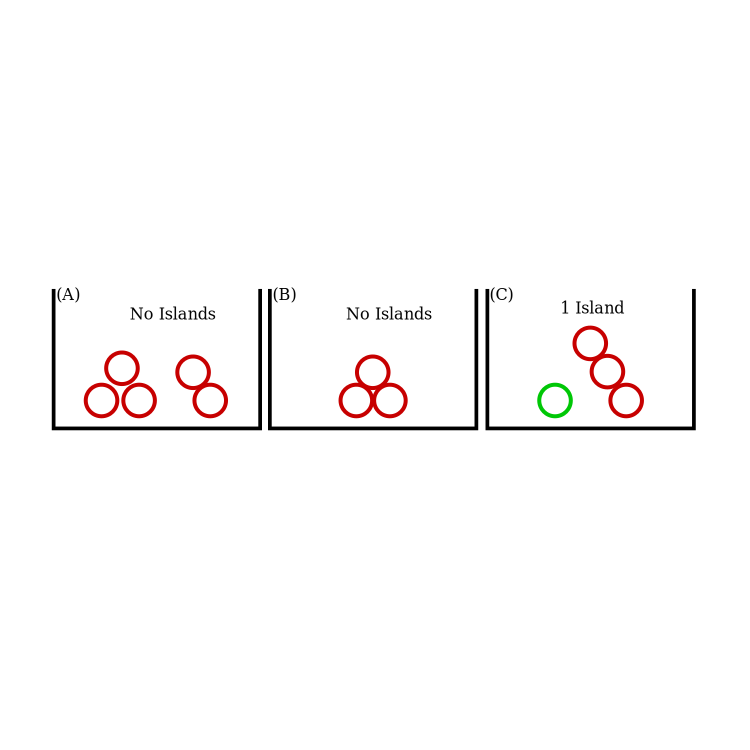
\includegraphics[width=0.8\textwidth]{islandExamples.png}
            \caption{Shows examples of what is considered an Island. In subfigure (A) there is no lone cup. Note also that even though the cups are not kissing, this is not considered a long island. In subfigure (B) is obvious to see there are no islands present. Subfigure (C) has 1 island highlighted in green.}
            \label{fig:islandExamples}
        \end{figure}

\section{Miscellaneous Rules}\label{sec:Misc}

	\subsection{Glitches in the Matrix}\label{ssec:Glitches}
		\subsubsection{}\label{sec:Misc,onto}
			 If a shot happens to land and stay on top of the cups, that shot will count as a miss.
             Congratulations - you are lucky, but you have not proved that you have any pong skills at all.
        \subsubsection{}\label{sssec:Misc,wind}
            When playing outside, and a gust of wind comes up and blows the ball causing a miss, that is unfortunate but valid.
            Vise versa for defenders.

	\subsection{Balling Your Own Cups}\label{ssec:OwnScore}
		\subsubsection{}\label{sssec:OwnScore,penalty}
             In the event that a player who has possession of the ball drops a ball into his own cups \emph{accidentally} that cup is removed as if a ball was just sunk by opponents.
             \footnote{This sinking does not count to the on-fire or heating up or double in for the other team.}
		\subsubsection{}\label{sssec:OwnScore,backboard}
			 In the event that a player who does not have possession of the ball comes in contact with the ball and as a result that ball is sunk in of their own cups, such as by unintentionally acting as a backboard, that shot IS counted and the cup is hit.
			 
	\subsection{During the Game}\label{ssec:DuringGame}
		\subsubsection{}\label{sssec:MaintainRack}
			During the game, players must maintain their rack.
            Meaning That they should keep the cups kissing with their neighbours, and two fingers from the edge but no more than 4.
            The remaining cups should be in the places they started the game in unless a valid rerack moved them.
		\subsubsection{}\label{sssec:Knockover}
			A team member knocking over their own cups also counts as a removal of that cup from the game as if a ball was sunk. no matter the reason.
		\subsubsection{}\label{sssec:swiping_no_bounce}
			A player that swipes/grabs a ball that has been thrown by the opponent and not yet bounced must then take a cup out of their rack of the opponents choice.
            The ball is not returned to the thorwer.
		\subsubsection{}\label{sssec:FinalCountDown}
			If both sides only have one cup left in their rack, the music must be changed to one of the following songs: The Final Count Down by Europe, Chariots of fire, the pong dance.
		\subsubsection{}\label{sssec:finalSongEnd}
			If the finally song ends (see \ref{sssec:FinalCountDown}) Then the teams switch sides and play anther song listed in. \ref{sssec:FinalCountDown}


% The End
\end{document}
